% $Header: /Users/joseph/Library/texmf/tex/latex/beamer/solutions/conference-talks/conference-ornate-20min.en.tex,v 90e850259b8b 2007/01/28 20:48:30 tantau $

\documentclass{beamer}
\graphicspath{{_plots/}}

\usepackage[makeroom]{cancel}
\usepackage{epstopdf}
\providecommand{\abs}[1]{\lvert#1\rvert}
\providecommand{\norm}[1]{\lVert#1\rVert}
%\newcommand{\rhoeq}{ \rho_{\mbox{eq}} }
\newcommand{\rhoeq}{ \rho_{\mbox{\scriptsize eq}} }
% This file is a solution template for:

% - Talk at a conference/colloquium.
% - Talk length is about 20min.
% - Style is ornate.



% Copyright 2004 by Till Tantau <tantau@users.sourceforge.net>.
%
% In principle, this file can be redistributed and/or modified under
% the terms of the GNU Public License, version 2.
%
% However, this file is supposed to be a template to be modified
% for your own needs. For this reason, if you use this file as a
% template and not specifically distribute it as part of a another
% package/program, I grant the extra permission to freely copy and
% modify this file as you see fit and even to delete this copyright
% notice.


\mode<presentation>
{
  \usetheme{Frankfurt}
  % or ...

  \setbeamercovered{transparent}
  % or whatever (possibly just delete it)
}


\usepackage[english]{babel}
% or whatever

\usepackage[latin1]{inputenc}
% or whatever

\usepackage{times}
\usepackage[T1]{fontenc}
% Or whatever. Note that the encoding and the font should match. If T1
% does not look nice, try deleting the line with the fontenc.


\title%[Short Paper Title] % (optional, use only with long paper titles)
{The f-wave method for nonlinear conservation laws with spatially varying flux}

%\subtitle
%{Include Only If Paper Has a Subtitle}

\author%[Author, Another] % (optional, use only with lots of authors)
{Xin Yang, Hai Zhu}
% - Give the names in the same order as the appear in the paper.
% - Use the \inst{?} command only if the authors have different
%   affiliation.

\institute[University of Washington] % (optional, but mostly needed)
{
%  \inst{1}%
  Course project for Amath 574\\
  Department of Applied Mathematics\\
  University of Washington
}
%  \and
%  \inst{2}%
%  Department of Theoretical Philosophy\\
%  University of Elsewhere}
% - Use the \inst command only if there are several affiliations.
% - Keep it simple, no one is interested in your street address.

\date[03/12/2015] % (optional, should be abbreviation of conference name)
{Mar 12 2015}
% - Either use conference name or its abbreviation.
% - Not really informative to the audience, more for people (including
%   yourself) who are reading the slides online

%\subject{Applied Mathematics}
% This is only inserted into the PDF information catalog. Can be left
% out.

% If you have a file called "university-logo-filename.xxx", where xxx
% is a graphic format that can be processed by latex or pdflatex,
% resp., then you can add a logo as follows:

% \pgfdeclareimage[height=0.5cm]{university-logo}{university-logo-filename}
% \logo{\pgfuseimage{university-logo}}



% Delete this, if you do not want the table of contents to pop up at
% the beginning of each subsection:
%\AtBeginSubsection[]
%{
%  \begin{frame}<beamer>{Outline}
%    \tableofcontents[currentsection,currentsubsection]
%  \end{frame}
%}


% If you wish to uncover everything in a step-wise fashion, uncomment
% the following command:

%\beamerdefaultoverlayspecification{<+->}

\begin{document}

\begin{frame}
  \titlepage
\end{frame}

\begin{frame}{Outline}
  \tableofcontents
  % You might wish to add the option [pausesections]
\end{frame}


% Structuring a talk is a difficult task and the following structure
% may not be suitable. Here are some rules that apply for this
% solution:

% - Exactly two or three sections (other than the summary).
% - At *most* three subsections per section.
% - Talk about 30s to 2min per frame. So there should be between about
%   15 and 30 frames, all told.

% - A conference audience is likely to know very little of what you
%   are going to talk about. So *simplify*!
% - In a 20min talk, getting the main ideas across is hard
%   enough. Leave out details, even if it means being less precise than
%   you think necessary.
% - If you omit details that are vital to the proof/implementation,
%   just say so once. Everybody will be happy with that.

\section{Review}
\subsection{The wave-propagation form}
\begin{frame}{Review on the wave-propagation form}
Given system of conservation laws
\[
q_t+f(q)_x=0,
\]
we have the discretization using the wave-propagation form:
\[
Q^{n+1}_i=Q^{n}_i-\frac{\Delta t}{\Delta x}\left(\sum (s^p)^+{\cal W}_{i-1/2}^p+\sum (s^p)^-{\cal W}_{i+1/2}^p\right)
\]
where ${\cal W}^p_{i-1/2}$ are the waves of discontinuities generated at the interface between cells $i-1$ and $i$
\end{frame}
\begin{frame}{Review on the wave-propagation form}
Generally, ${\cal W}^p_{i-1/2}$ is obtain by decomposing the jumps $Q_i^n-Q_{i-1}^n$ into the eigenvectors of some matrix $A$ approximating the Jacobian matrix $ \nabla_q f(q) $
\[
Q_i^n-Q_{i-1}^n=\sum {\cal W}^p_{i-1/2}=\sum \alpha^p r^p
\]
\end{frame}
\subsection{Problems in variable coefficient cases}
\begin{frame}{Problems in variable coefficient cases}
Consider generalized Riemann problem
\begin{align*}
	\begin{cases}q_t+(u_l q)_x=0 & \text{if } x<0 \\
	q_t+(u_r q)_x=0 & \text{if } x>0\end{cases}, \,\,\,
	q(x,0)=\begin{cases}q_l & \text{if } x<0 \\
	q_r & \text{if } x>0\end{cases}
\end{align*}
\begin{figure}
  \centering
  % Requires \usepackage{graphicx}
  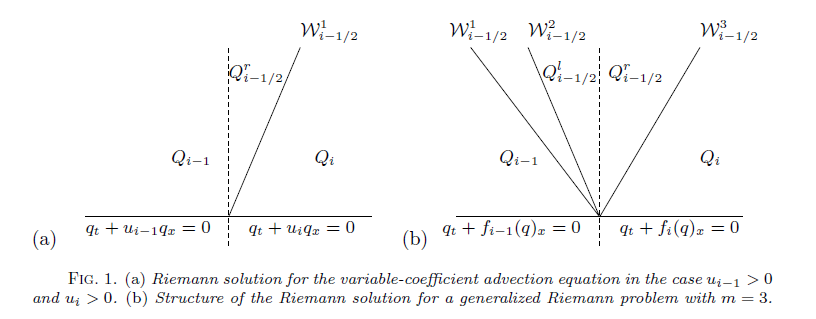
\includegraphics[width=\textwidth]{discon.png}\\
\end{figure}
\cite[p. 960]{bale2002}
\end{frame}

\section{The f-wave method}
\subsection{Definition}
\begin{frame}{What is the f-wave method?}
Flux differencing form:
\[
Q^{n+1}_i=Q^n_i-\frac{\Delta t}{\Delta x}\left( f(Q_{i+1/2})-f(Q_{i-1/2})\right)
\]
we call the wave ${\cal W}$ w-waves. If instead we decompose the difference of flux, we get f-waves ${\cal Z}^p_{i-1/2}$.
\begin{align*}
f(Q_i)-f(Q_{i-1})=\sum \beta^p_{i-1/2} r^p_{i-1/2}\equiv \sum {\cal Z}^p_{i-1/2}.
\end{align*}
\end{frame}

%\begin{frame}{Implementation}
%1.2..3...
%\end{frame}
\subsection{Advantages}
\begin{frame}{Why f-waves?}
\begin{itemize}
\item Easy to implement.
\item Better conservation.
\item Directly generalized to the case with source term.
\item May be a more fundamental object.
\end{itemize}
\end{frame}

\begin{frame}{Conservation: Roe condition}
For the standard w-wave propagation form, an approximate Riemann solver is conservative iff
\begin{align*}
A_{i-1/2}(Q_i-Q_{i-1})=f_{i}(Q_i)-f_{i-1}(Q_{i-1})
\end{align*}
is satisfied. However, the conservation is a natural result in the f-wave method
\begin{align*}
Q_i^{n+1}=Q_i^{n}-\frac{\Delta t}{\Delta x}\left[\sum sign((\lambda^p)^-) {\cal Z}_{i+1/2}^p+\sum sign((\lambda^p)^+) {\cal Z}_{i-1/2}^p\right] \\
Q_{i+1}^{n+1}=Q_{i+1}^{n}-\frac{\Delta t}{\Delta x}\left[\sum sign((\lambda^p)^-) {\cal Z}_{i+3/2}^p+\sum sign((\lambda^p)^+) {\cal Z}_{i+1/2}^p\right]
\end{align*}
\end{frame}

\begin{frame}{Convergence study}
\begin{figure}
  \centering
  % Requires \usepackage{graphicx}
  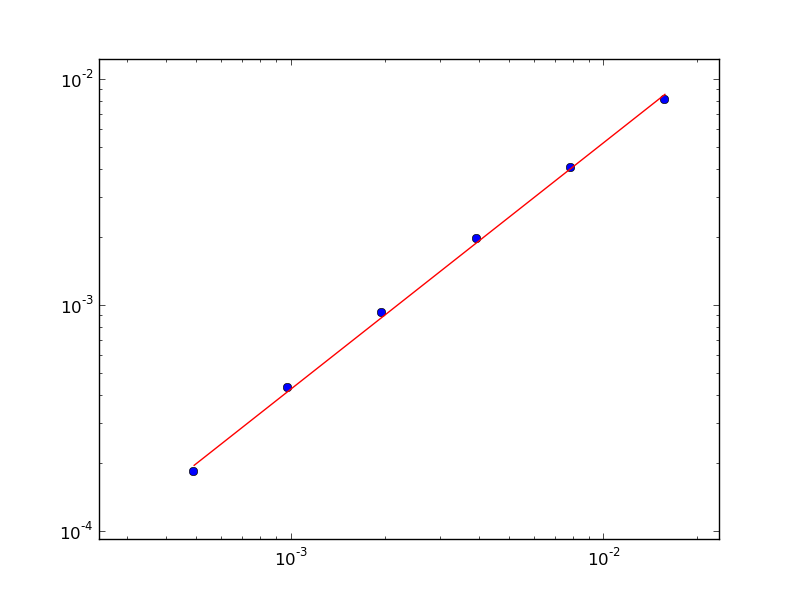
\includegraphics[width=0.8\textwidth]{loglog_error.png}\\
  \caption{$L_1$ error versus cell length. Second order accuracy is obtained for smooth solution.}\label{conv}
\end{figure}

\end{frame}

\section{Nonlinear elastic waves in layered media}
\subsection{Model setup}
\begin{frame}{1D Elastic wave equations}
\begin{align*}
\epsilon(x,t)_t-u(x,t)_x=0 \\
\rho(x) u(x,t)_t-\sigma(\epsilon,x)_x=0
\end{align*}
The first equation is definition of strain. The second one is the the Newton's second law. We shall consider a nonlinear model with exponential relation
\begin{align*}
\sigma(x,t)=\exp(K(x)\epsilon(x,t))-1
\end{align*}
in (Periodically) layered media
\begin{align*}
K(x)=\left\{
\begin{array}{cc}
K_A & \mbox{if }j\delta<x<(j+\alpha)\delta \mbox{ for some integer } j,\\
K_B & \mbox{otherwise.}
\end{array}
\right.
\end{align*}
\end{frame}

\begin{frame}{Structure of solution to the Riemann problem}
The Jacobian
\begin{align*}
f_q(q,x)=\left(
                     \begin{array}{cc}
                       0  &  -\frac{1}{\rho}\\
                       -\sigma_{\epsilon}(\epsilon,x) &  0 \\
                     \end{array}
                   \right).
\end{align*}
Sound speed (eigenvalues)
\begin{align*}
c(q,x)=\sqrt{\frac{\sigma_{\epsilon}(\epsilon,x)}{\rho(x)}}  \Longrightarrow \mbox{No transonic rarefaction wave}
\label{sounds}
\end{align*}
Therefore no entropy fix is required and we can choose the solution to the Riemann problem to be all shock solution.
\end{frame}

\begin{frame}{Approximate Riemann solver}
Eigenvectors are
\begin{align*}
r^1(q,x)=\left(
                     \begin{array}{c}
                       1 \\
                       Z(q,x)
                     \end{array}
                   \right)  ,\,\,\, \mbox{for } s^1(q,x)=-\sqrt{\frac{\sigma_{\epsilon}(\epsilon,x)}{\rho(x)}}
\end{align*}
\begin{align*}
r^2(q,x)=\left(
                     \begin{array}{c}
                       1 \\
                       -Z(q,x)
                     \end{array}
                   \right)  ,\,\,\, \mbox{for } s^2(q,x)=\sqrt{\frac{\sigma_{\epsilon}(\epsilon,x)}{\rho(x)}}
\end{align*}
where $Z(q,x)=\rho(x)c(q,x)$ is the impedance.
\end{frame}

\begin{frame}{Approximate Riemann solver}
Instead of giving the approximate Jacobian $A_{i-1/2}$ directly, we specify the eigenvalues and eigenvectors of $A_{i-1/2}$:
\begin{align}
r^1_{i-1/2}=r^1_{i-1}=\left[
                        \begin{array}{c}
                          1 \\ Z_{i-1} \\
                        \end{array}
                      \right], & \,\,\, s^1_{i-1/2}=-\sqrt{\frac{\sigma'_{i-1}(\epsilon_{i-1})}{\rho_{i-1}}}\\
r^2_{i-1/2}=r^2_{i}=\left[
                        \begin{array}{c}
                          1 \\ -Z_{i} \\
                        \end{array}
                      \right], &\,\,\, s^2_{i-1/2}=-\sqrt{\frac{\sigma'_{i}(\epsilon_{i})}{\rho_{i}}}
\end{align}
Here we are using eigenvalues and eigenvectors according to the cells where they are.
\end{frame}
\subsection{Simulations}
\begin{frame}{Homogeneous; speed, impedance mismatch}
\begin{figure}
  % Requires \usepackage{graphicx}
  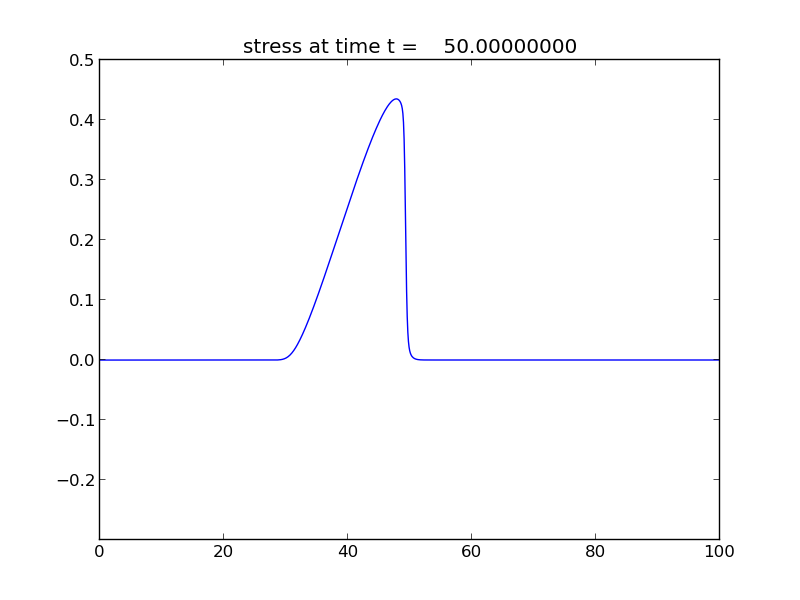
\includegraphics[width=0.3\textwidth]{homo1.png}
  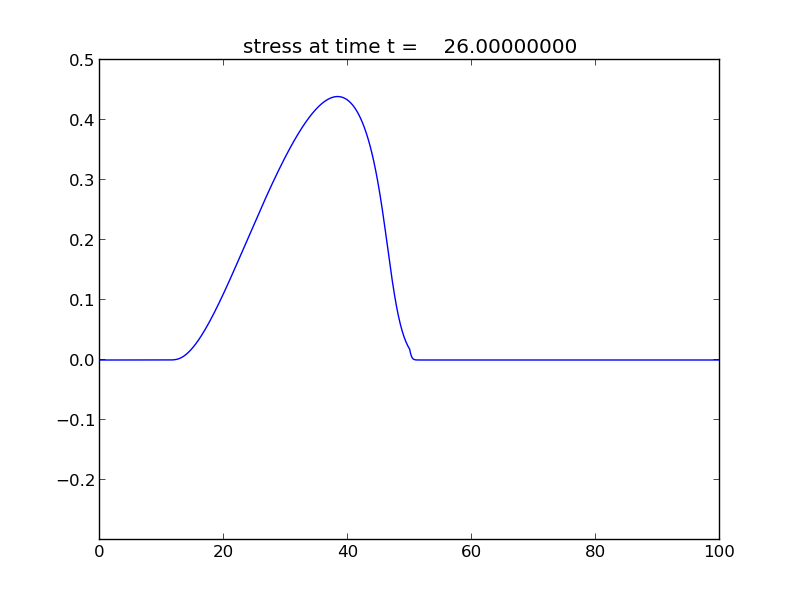
\includegraphics[width=0.3\textwidth]{sound1.png}
  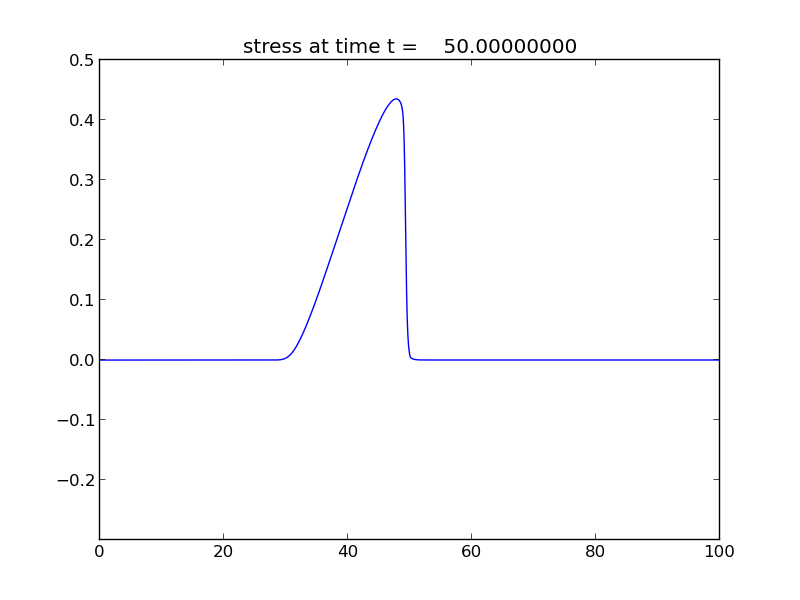
\includegraphics[width=0.3\textwidth]{reflect1.png}\\
 % 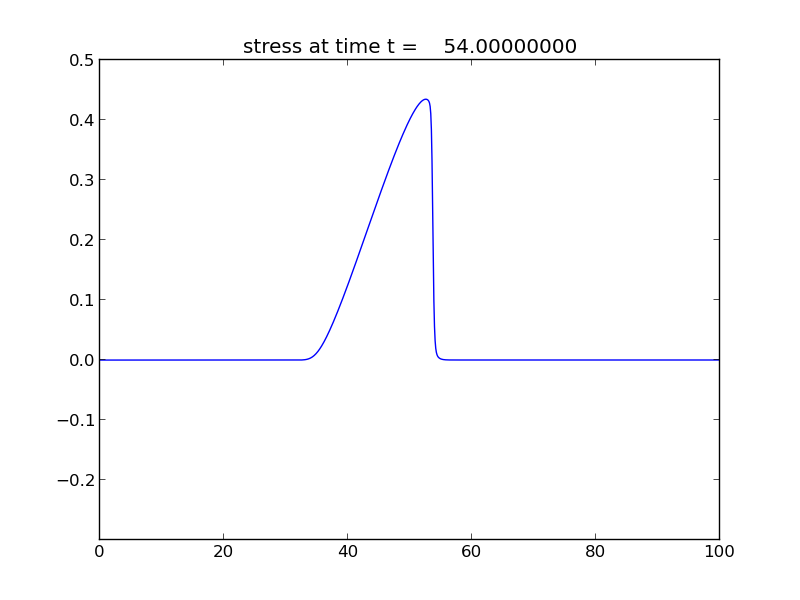
\includegraphics[width=0.3\textwidth]{homo2.png}
 % 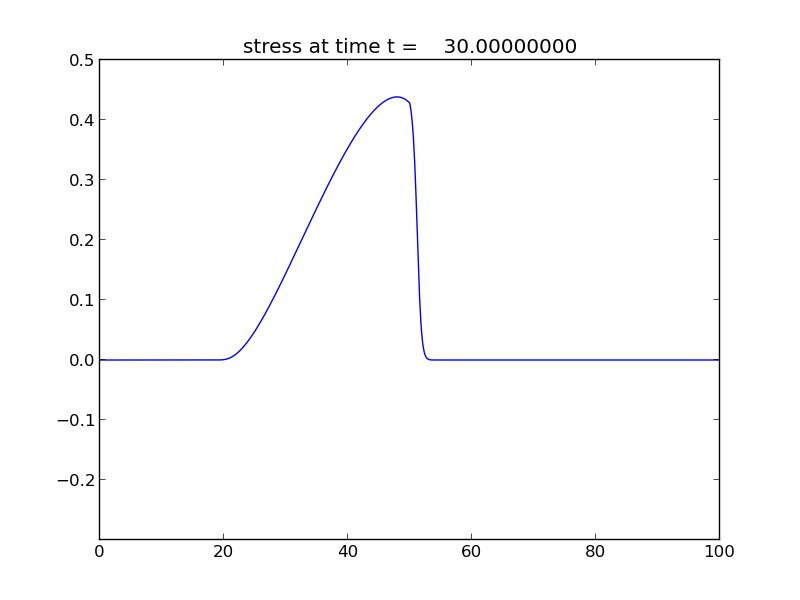
\includegraphics[width=0.3\textwidth]{sound2.png}
 % 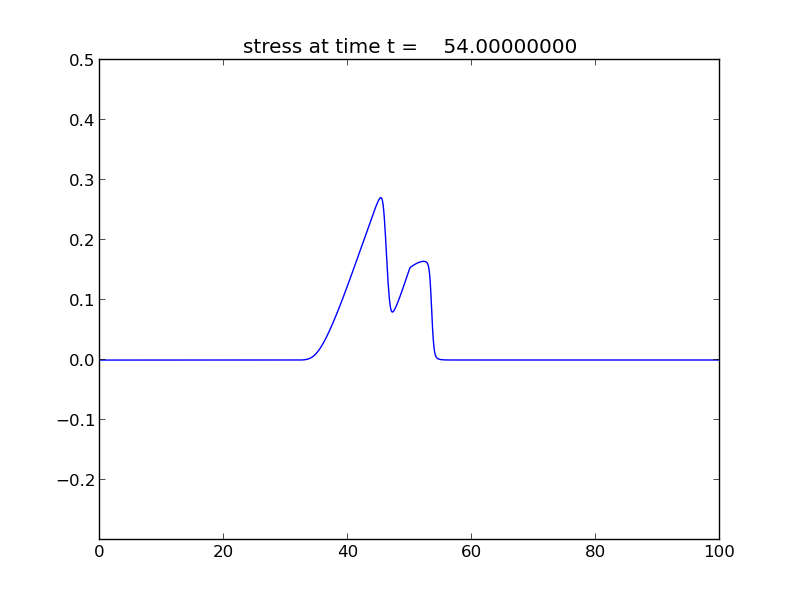
\includegraphics[width=0.3\textwidth]{reflect2.png}\\
  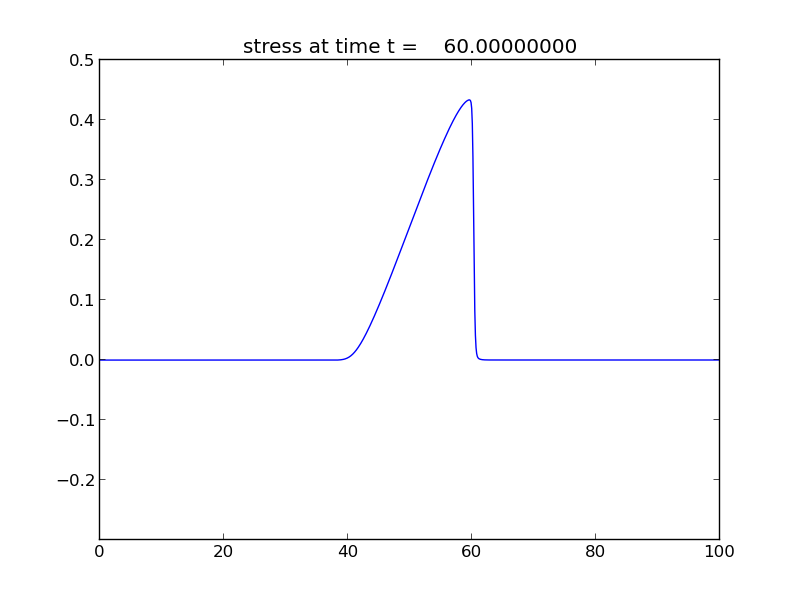
\includegraphics[width=0.3\textwidth]{homo3.png}
  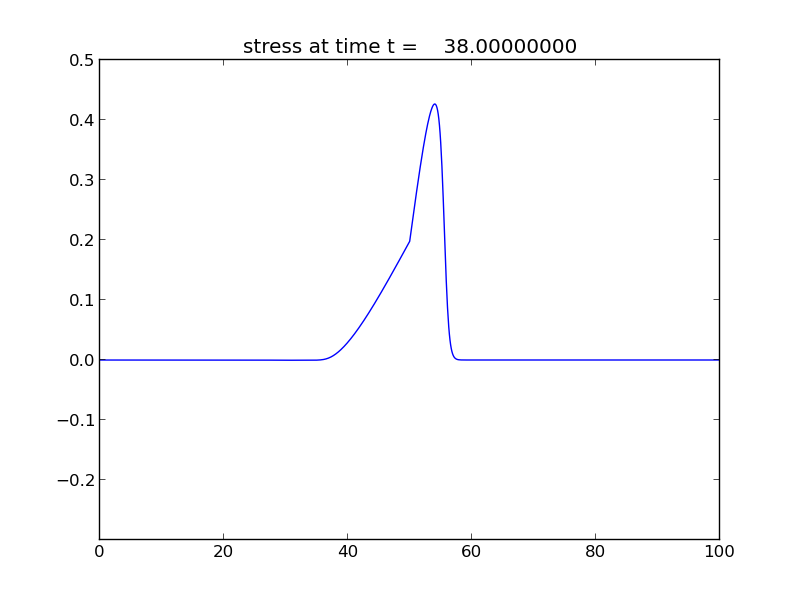
\includegraphics[width=0.3\textwidth]{sound3.png}
  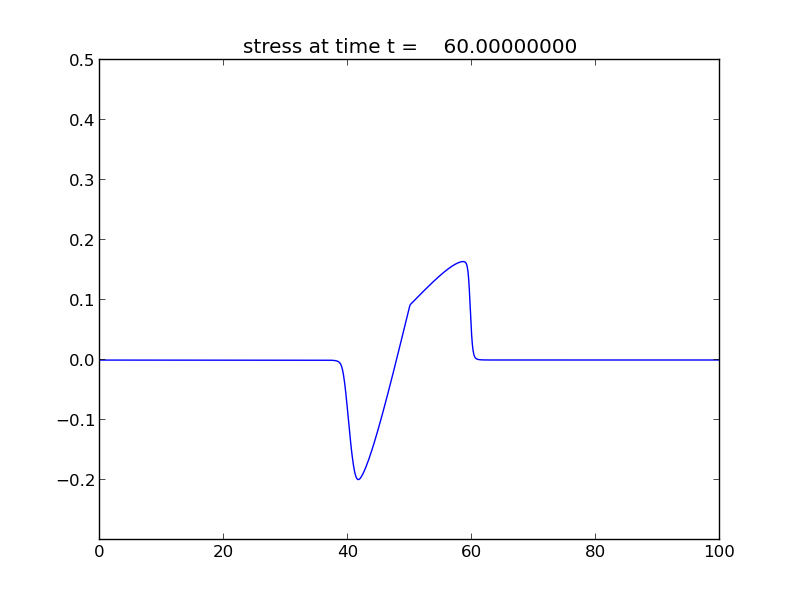
\includegraphics[width=0.3\textwidth]{reflect3.png}\\
    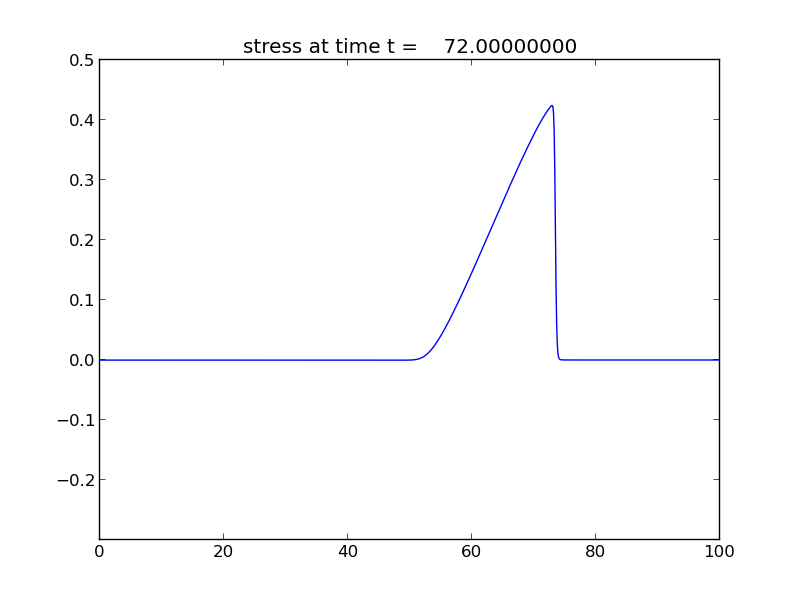
\includegraphics[width=0.3\textwidth]{homo4.png}
  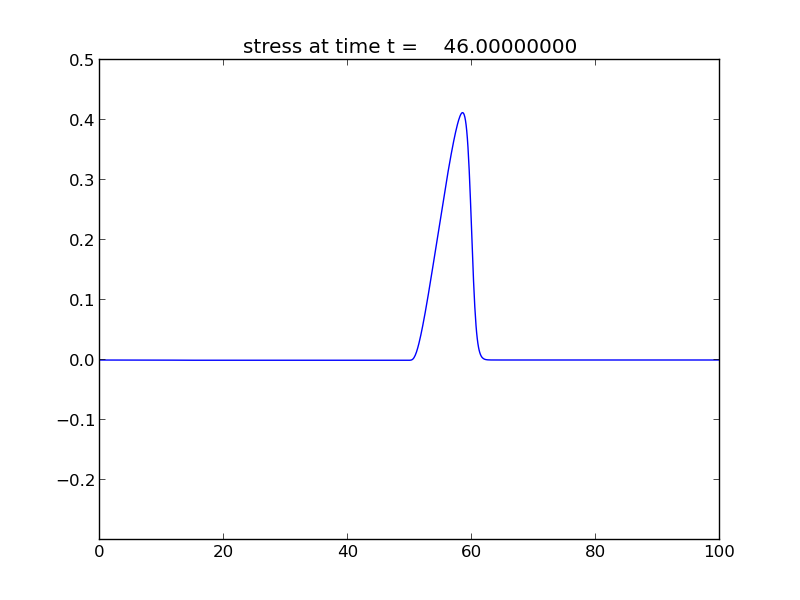
\includegraphics[width=0.3\textwidth]{sound4.png}
  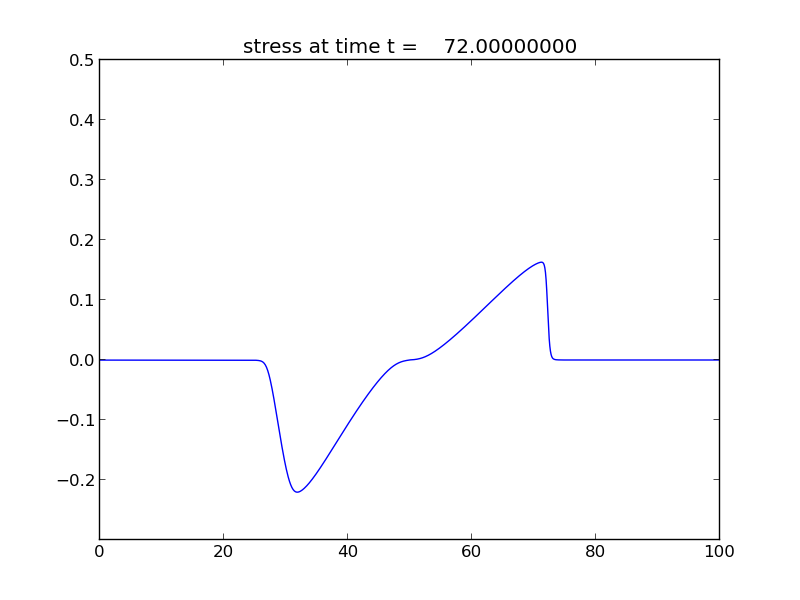
\includegraphics[width=0.3\textwidth]{reflect4.png}
  \caption{The wave travelling through the interface (at $x=50$) of two materials. Left column: two homogeneous materials with the same impedance and sound speed. Middle column: two homogeneous materials with the same impedance and different sound speeds. Right column: two homogeneous materials with different impedances and the same sound speed.}
  \label{imp}
\end{figure}
\end{frame}

\begin{frame}{Generation of solitons in layered media}
Strain and stress waves
\begin{figure}
  % Requires \usepackage{graphicx}
  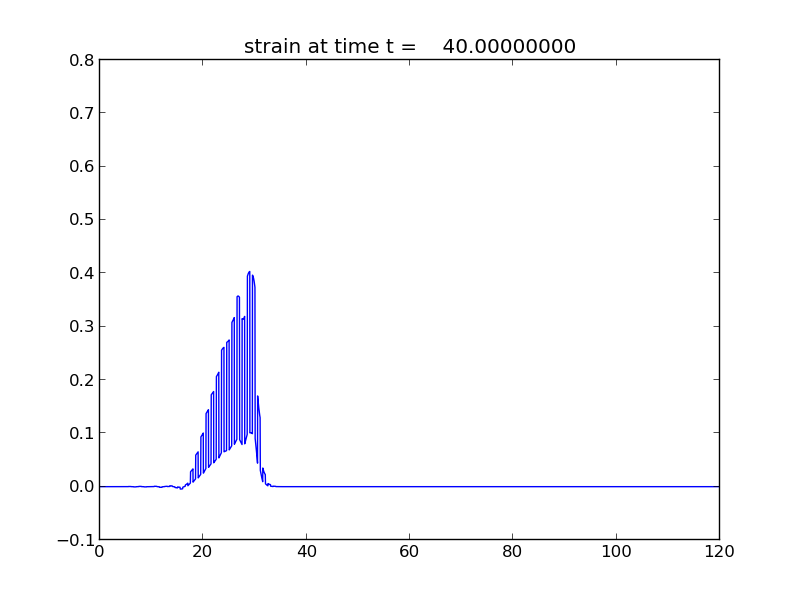
\includegraphics[width=0.35\textwidth]{frame0004fig1.png}
  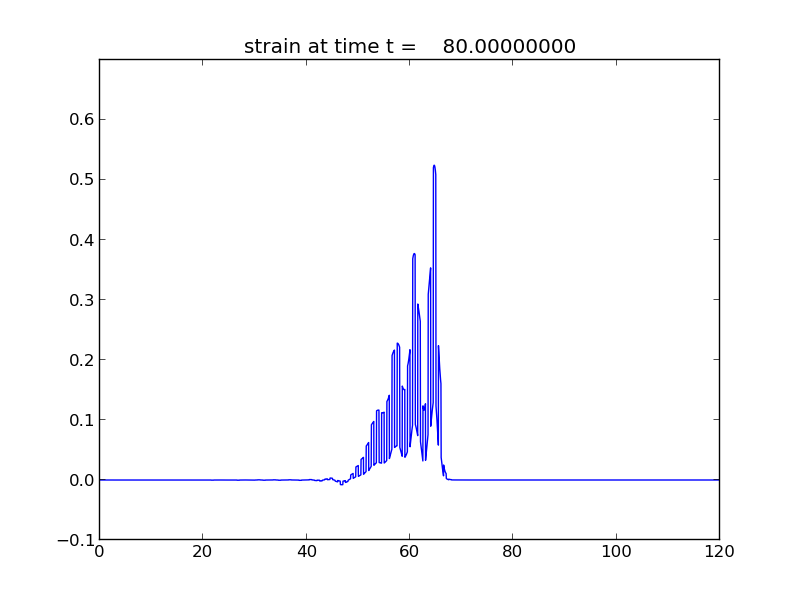
\includegraphics[width=0.35\textwidth]{frame0008fig1.png}
  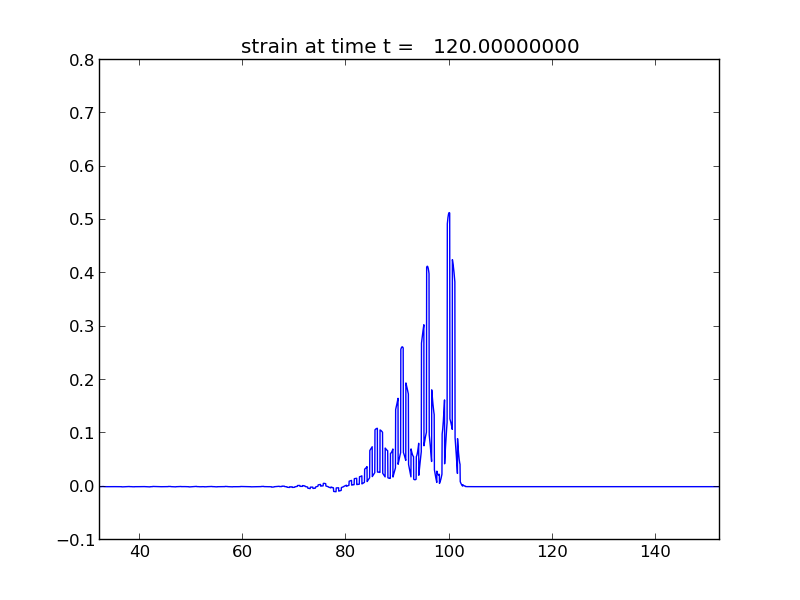
\includegraphics[width=0.35\textwidth]{frame0012fig1.png}\\
  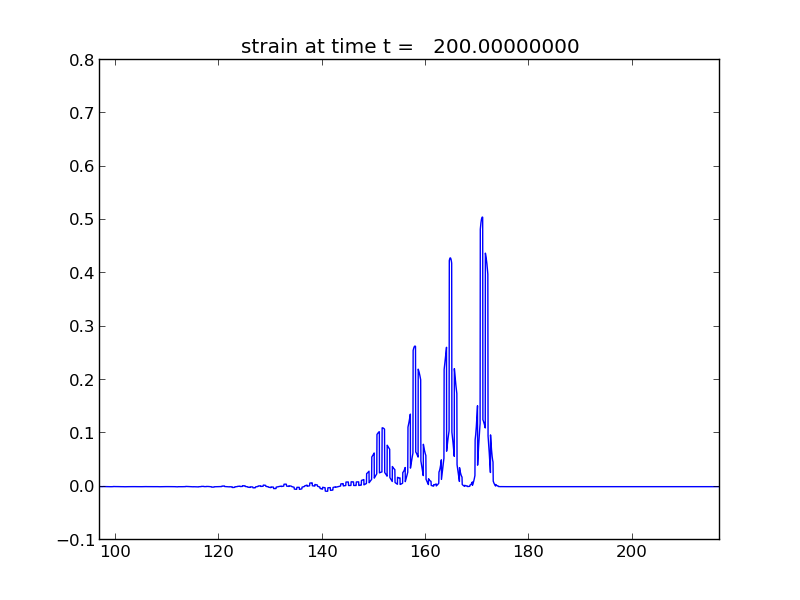
\includegraphics[width=0.35\textwidth]{frame0020fig1.png}
  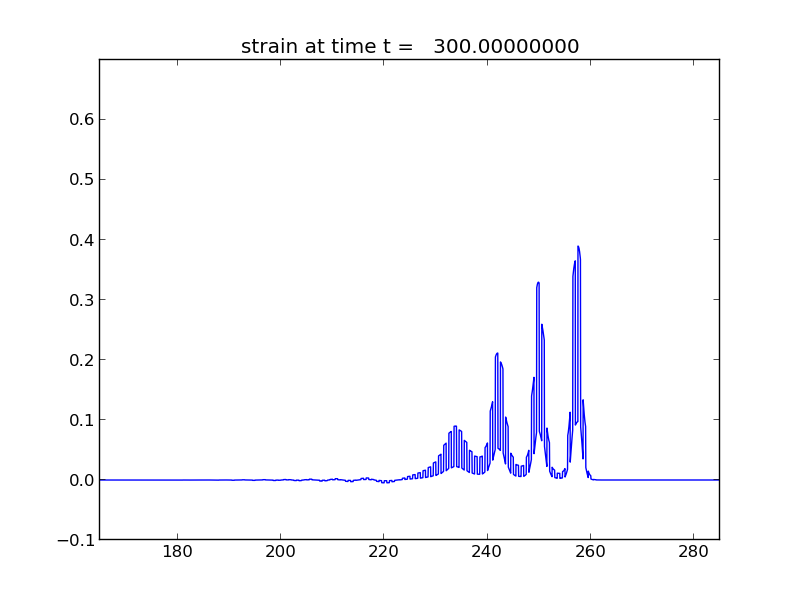
\includegraphics[width=0.35\textwidth]{frame0030fig1.png}
  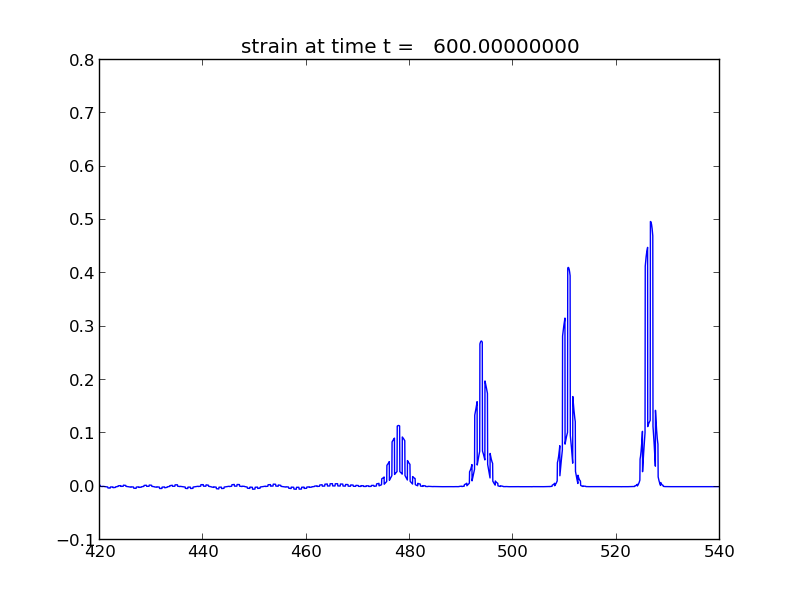
\includegraphics[width=0.35\textwidth]{frame0060fig1.png}
  %\caption{The decomposition of the initial single bump into soliton-like waves.}
  %\label{travelw}
\end{figure}
\end{frame}

\begin{frame}[fragile]{Stegosaurus}
\begin{figure}
  \centering
  % Requires \usepackage{graphicx}
  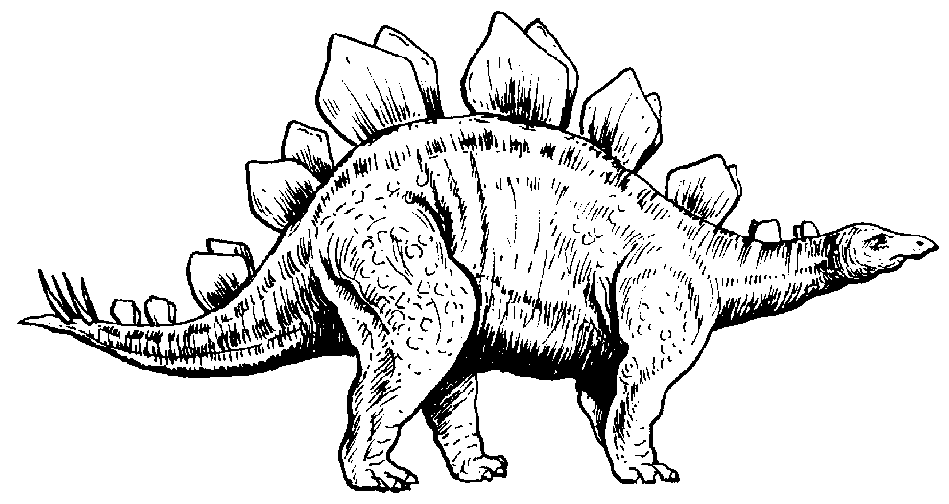
\includegraphics[width=\textwidth]{stegosaurus.png}\\
\end{figure}

\begin{verbatim}
From http://ancientadventurescambodia.com
/tag/stegosaurus/
\end{verbatim}

\end{frame}

\begin{frame}{Question session}
Thanks for listening. Questions?
\end{frame}



% All of the following is optional and typically not needed.
\appendix
\section<presentation>*{\appendixname}
\subsection<presentation>*{For Further Reading}

\begin{frame}[allowframebreaks]
  \frametitle<presentation>{References}
  \begin{thebibliography}{10}
%  \beamertemplatebookbibitems
  % Start with overview books.
  \bibitem{bale2002}
  D. S. Bale, R. J. LeVeque, S. Mitran, and J. A. Rossmanith, SIAM J. Sci. Comput 24 (2002), 955-978.
  \bibitem{leveque2002}
  Finite Volume Methods for Nonlinear Elasticity in Heterogeneous Media
  by R. J. LeVeque, Int. J. Numer. Meth. Fluids 40 (2002), pp. 93-104.
  \bibitem{leveque2003}
  Randall J. LeVeque and Darryl H. Yong, SIAM J. Appl. Math., 63 (2003), pp. 1539-1560.
  \bibitem{ketcheson2012}
  David I Ketcheson, Randall J. LeVeque Comm. Math. Sci. 10 (2012), pp. 859-874.
  \end{thebibliography}
\end{frame}
\end{document}


